\documentclass[letterpaper, 10pt, journal]{IEEEtran}
\usepackage{graphicx}
\usepackage{float}
\usepackage{listings}
\usepackage{color}
\usepackage{multirow}
\usepackage[table,xcdraw]{xcolor}
\usepackage[justification=centering]{caption}
\usepackage[spanish]{babel}
\selectlanguage{spanish}
\usepackage[utf8]{inputenc}
% Paquete para referenciar figuras
\usepackage{nameref}
\graphicspath{ {./Images/} }
% Paquetes para las funciones matematicas
\usepackage{amsmath}
\usepackage{amssymb}

\usepackage[justification=centering]{caption}
\lstset{frame=tb,
  language=Java,
  aboveskip=3mm,
  belowskip=3mm,
  showstringspaces=false,
  columns=flexible,
  basicstyle={\small\ttfamily},
  numbers=none,
  numberstyle=\tiny\color{gray},
  keywordstyle=\color{blue},
  commentstyle=\color{dkgreen},
  stringstyle=\color{mauve},
  breaklines=true,
  breakatwhitespace=true,
  tabsize=3
}

\begin{document}
\title{Tarea 2 - 10 Experimentos Cient\'ificos Mas Bellos De La Historia }
\author{Kathy~Brenes~Guerrero, Barnum~Castillo~Barquero

~\IEEEmembership{
    \begin{center}
        Maestr\'ia en Ciencias de la Computaci\'on, Introducci\'on a la Investigaci\'on, ITCR
    \end{center}
}}% <-this % stops a space

% The paper headers
\markboth{Instituto Tecnol\'ogico de Costa Rica, Introducci\'on a la Investigaci\'on, Octubre~2018}%
{Shell \MakeLowercase{\textit{et al.}}: Tarea 2 - 10 Experimentos Cient\'ificos Mas Bellos De La Historia }
\maketitle

\begin{IEEEkeywords}

\end{IEEEkeywords}

\section{Introducci\'on}
El siguiente reporte detalla 10 experimentos considerados por nosotros como los mejores de algunas revistas de divulgacion cient\'ifica, que forman parte de los “10 experimentos cien\'ificos mas bellos de la historia”.

\section{Ca\'ida libre de los cuerpos realizado por Galileo en el siglo XVI}

\subsection{Historia de Galileo}

Galileo Galilei nació en Pisa el 15 de febrero de 1564, solo tres días antes de la muerte de Miguel Ángel, el último de los héroes del alto Renacimiento, a los 89 años de edad. Se cree que la familia de Galileo procedía del Mugello, un valle apartado a 24 kilómetros por caminos montañosos hacia el norte desde Florencia. Esta pequeña región aislada debió de contar con una despensa de genes notables, pues de allí salieron también los artistas Fra Angelico y Giotto, así como la familia Médicis. \cite{[1]}
\newline
El padre de Galileo, Vincenzo, procedía de una familia noble florentina que había conocido mejores tiempos. Tenía poco dinero y un carácter combativo que contribuía a mantenerle en esa situación. Pero era también un hombre de verdadero talento, había estudiado música en Venecia y se había convertido en un eminente experto en teoría musical. Se rebeló contra la camisa de fuerza del contrapunto, insistiendo en que la música debía agradar al oído en la práctica antes que a la mente en la teoría formal de la partitura. Sus composiciones influyeron en la liberación musical que desembocaría en el nacimiento de la ópera al final del siglo. \cite{[2]}
\newline
De tal palo, tal astilla. Galileo se convirtió en un mozo pelirrojo espabilado y presuntuoso cuya fachada encantadora y extrovertida ocultaba un temperamento algo más complejo. En casa, las cosas no eran fáciles. Su madre, Giulia, consideraba que se había casado por debajo de sus posibilidades. Con un inútil, decía ella. Esto no tardó en amargarla, convirtiéndola en una esposa regañona y una madre absorbente. Galileo se acostumbró a ser el centro de su atención, beneficiándose de la autoestima resultante, pero tras su carácter exuberante acechaban siempre las incertidumbres nacidas de su tormentosa vida familiar. \cite{[2]}
\newline
Cuando Galileo contaba diez años la familia se trasladó a Florencia, donde su padre se convirtió en músico de la corte y conocido polemista. Galileo fue enviado a educarse al monasterio de Vallombrosa, en los montes, a 24 kilómetros al este de la ciudad. 
\newline
En 1581, a los 17 años, Galileo volvió a su ciudad natal para estudiar medicina en la Universidad de Pisa. Su padre quería que se hiciera médico para que aportara unos muy necesarios ingresos a la familia.
\newline
Galileo adquirió la costumbre de colarse en las conferencias de Ricci, destinadas a los jóvenes de la corte. El intruso se armó de valor y se dirigió al maestro, haciéndole preguntas al acabar las conferencias. Ricci percibió enseguida su talento excepcional y le animó.
\newline
Galileo había encontrado por fin un maestro al que podía admirar. Ricci no era un matemático cortesano cualquiera. Era también un ingeniero militar excepcional. (Algunos años más tarde fue el encargado de reconstruir la fortaleza-islote del Château d’If frente a Marsella, cuyas fortificaciones describe Alejandro Dumas en su famosa novela, El Conde de Montecristo.) Ricci era la prueba de que se podía ganar dinero con las matemáticas si se destinaban a fines prácticos. \cite{[2]}
\newline
A Vincenzo no le hizo gracia enterarse de la escasa atención que su hijo dedicaba a sus estudios de medicina, pero ya empezaba a aceptar que este nunca sería médico: carecía del temperamento adecuado. Cuando la corte volvió a Florencia, Vincenzo abordó a Ricci y le preguntó si podría dar lecciones a Galileo. Ricci comenzó su instrucción con Euclides y Arquímedes. La claridad y el rigor de las argumentaciones de Euclides fueron una revelación para Galileo. Mientras que las argumentaciones escolásticas tradicionales apelaban a autoridades establecidas como la de Aristóteles, la autoridad para Euclides era la verdad, y solo esta se consideraba suficiente para probar sus proposiciones. En sus Elementos Euclides sentó las bases de la geometría y esbozó el método que habrían de adoptar los matemáticos. Comenzando por las definiciones más simples y evidentes en sí mismas (el punto, la línea) procedía luego a los teoremas, demostrando rigurosamente cada uno, que partía del anterior y así sucesivamente, construyendo de este modo el irrefutable edificio de la geometría.\cite{[1]}
\newline
Galileo no tardó en demostrar su talento excepcional en la esfera práctica. Como reza la historia muchas veces contada, un domingo, mientras escuchaba un largo sermón en la catedral de Pisa, se sintió intrigado por el balanceo de una lámpara sujeta al techo por medio de un largo alambre. Se percató de que la lámpara siempre tardaba el mismo tiempo en completar una oscilación, sin importar la amplitud del arco descrito en cada balanceo. En un arrebato de inspiración Galileo se dio cuenta de que se comportaba como el pulso. En cuanto llegó a casa construyó un péndulo con un hilo y una pesa de plomo. Realizó una serie de experimentos con diferentes pesos y diferentes longitudes de hilo. A partir de estos experimentos fabricó un aparato que podía usarse para tomar el pulso a un paciente. Lo mostró a algunos miembros del departamento de medicina de la universidad y quedaron tan impresionados que le robaron la idea de inmediato. Lo que obtuvo Galileo del pulsilogium, como vino a llamarse, fue un cierto renombre local. Cuando empezó a usarse en muchas otras ciudades italianas, Galileo no recibió dinero ni tampoco crédito por el invento. (El concepto de ley de patentes era todavía ajeno a la Italia del siglo XVI. El secreto, el plagio, el espionaje y la falsificación se consideraban parte del proceso de manufactura.)\cite{[2]}
\newline
Como resultado de esta práctica comercial, más otras a las que se entregaba Galileo en las tabernas, se le acabó el dinero. En 1685, después de cuatro años de universidad, volvió sin título a su casa de Florencia. Pero la falta de titulación no era suficiente para desanimar a alguien con tanta confianza en sí mismo. Se estableció enseguida como matemático, dando clases particulares cuando y donde podía. \cite{[1]}
\newline
La admiración de Galileo por los antiguos seguía intacta, pero no era nada propenso a la reverencia acrítica. Por esta época publicó una obra breve titulada La Balancietta.En ella describió el famoso experimento hidrostático realizado para determinar la cantidad de oro y plata empleadas en la manufactura de la corona de oro del rey Hierón (que según el fraudulento orfebre era de oro macizo). Después, Galileo tuvo la audacia de hacer mejoras sobre el experimento de Arquímedes, describiendo un método mucho mejor para determinar las proporciones de los distintos metales, empleando una balanza hidrostática de su propia invención. La balanza, conocida como balancietta, era un instrumento extremadamente delicado del mayor refinamiento técnico, capaz de detectar diferencias minúsculas de peso. Característico tanto de su época como de su inventor, era también un instrumento de gran belleza. Como su anterior pulsilogium, causó gran asombro a lo largo y ancho de Italia, pero una vez más la recompensa de Galileo fue una fama pasajera y no la fortuna. (Cada vez era más obvio su anhelo tanto de gloria como de riqueza.)\cite{[2]}
\newline
En muchos aspectos Galileo seguía siendo un hombre medieval. Su aceptación del pensamiento de la época, la autoridad de la iglesia e incluso de los cuentos de hadas literarios no se vio sacudida por su creciente conciencia científica. Su desprecio hacia la autoridad se restringía al único terreno en el que sabía lo que decía y sus oponentes no. En su mente coexistían lo medieval y lo moderno. De hecho, este conflicto entre dos mundos que no encajaban puede muy bien haber sido una fuente de estímulo. Shakespeare, contemporáneo de Galileo, tenía una mente similarmente dividida, y una actitud aún más esquizoide es manifiesta en su sucesor Newton, cuyo logro intelectual supremo fue mantener una firme creencia tanto en el mundo matemático de la astronomía como en el mundo mágico de la alquimia.\cite{[1]}
\newline
Había estudiado las obras de Arquímedes Del equilibrio de los planos y De conoides y esferoides. La primera era la obra seminal de la mecánica en la que Arquímedes formuló su «ley de la palanca»; en la segunda puso en práctica la ley que determina el centro de gravedad de una serie de paraboloides (el sólido formado al rotar una parábola sobre su eje). Genio y figura, Galileo se propuso aventajar a su héroe con el hallazgo de una manera práctica y original de descubrir el centro de gravedad de diversos esferoides. Galileo tardaría muchos años en publicar estos trabajos, pero circularon en forma manuscrita entre matemáticos de toda Italia, algunos de los cuales quedaron tan impresionados que tildaron a Galileo de «nuevo Arquímedes». Uno de ellos fue un marqués toscano llamado Guidobaldo del Monte, quien solo un año antes había publicado un extenso tratado de mecánica. Guidobaldo no era ningún diletante matemático (su tratado sería la obra fundamental sobre mecánica durante el siglo siguiente), y también estaba interesado en el centro de gravedad de los sólidos. Galileo fue a visitar a Guidobaldo y no tardaron en hacerse amigos. Compartieron sus hallazgos sobre la determinación de los centros de gravedad y Guidobaldo, muy impresionado, llamó la atención del nuevo gran duque de Toscana sobre la persona de Galileo.\cite{[2]}
\newline
El interés de los mecenas aristocráticos tiende a ser volátil, pero este no habría de ser el caso de Guidobaldo. Galileo había encontrado al fin un padrino constante y firme en su apoyo. Al quedar vacante el puesto de profesor de matemáticas en Pisa, Guidobaldo recomendó a Galileo de inmediato, y fue aceptado. Galileo reaccionó con júbilo. Al fin lo había conseguido. Solo después descubrió que su salario era de solo 60 coronas, más o menos lo que ganaba un tendero, y apenas suficiente para mantener a un hombre de las crecientes aspiraciones, apetitos y tamaño de Galileo. \cite{[2]}
\newline
La Universidad de Pisa no estaba preparada para el regreso de su díscolo hijo. El nuevo profesor de matemáticas (que no había logrado obtener un título en esta misma universidad) llegó con renovada confianza en sí mismo. Con sus 25 años, su abundante cabello rojo y su gusto por la controversia, se convirtió rápidamente en una figura popular, al menos entre los estudiantes.\cite{[2]}

\subsection{Experimento}
Galileo realizó su legendario experimento desde lo alto de la torre inclinada de Pisa, que confirmó su intuición previa acerca del granizo. Dejó caer dos objetos del mismo material y diferente peso, y cayeron a la misma velocidad. El más pesado no cayó a mayor velocidad, como debería haber hecho según Aristóteles.
\newline
El episodio es coherente no solo desde un punto de vista científico, sino también con la personalidad del protagonista, aunque la evidencia de que realmente tuviera lugar es tan nebulosa como la teoría que pretendía desacreditar. Aunque solo sea por su ejemplaridad merece consideración. Galileo quiso realizar una demostración pública de un error de Aristóteles, lo que ya es de por sí significativo dado que las enseñanzas de Aristóteles se consideraban como de una pieza, científicamente hablando. Cada elemento, cada ley, cada suposición se tenían por conexas entre sí. Al demostrar la falsedad de una de las partes, Galileo parecía sugerir la falsedad del todo, aunque no fuera esa su intención.
\newline
Como veremos, Galileo no pretendía tal osadía. A lo que se oponía en realidad era a la actitud aristotélica de fondo. La ciencia trata de los fenómenos de la realidad, y estos son mejor aprehendidos por la experiencia que por principios del pensamiento. Primero debía venir el experimento y, solo después, debía seguir la teoría. Llegados a este punto conviene señalar que Galileo nunca llegó a descubrir por qué los dos cuerpos caían a la misma velocidad. Esto no fue explicado hasta un siglo más tarde, cuando New¬ton formuló su ley de la gravedad: todo cuerpo en el universo atrae a otro a una fuerza que varía en proporción directa a sus respectivas masas y de modo inversamente proporcional al cuadrado de la distancia entre ellos. El mérito de Galileo es que recurrió a los resultados de la experiencia en lugar de a la teoría.
\newline
La trascendencia de lo que Galileo estaba haciendo era mucho más radical de lo que él estaba dispuesto a admitir, incluso para sus adentros, al menos en un comienzo. Pese a sus alardes públicos desde la torre inclinada, siguió dando lecciones sobre la física de Aristóteles. Esto no respondió a una actitud hipócrita ya que, en gran parte, parece haber creído en lo que enseñaba. Tomemos su visión del universo, por ejemplo. Copérnico había publicado ya en 1543, su propia teoría, en la que describía cómo los planetas giraban alrededor del Sol. Es seguro que Galileo sabía de esto, pero seguía creyendo en el modelo aristotélico establecido por Ptolomeo, con la Tierra firmemente colocada en el centro del universo y el Sol, la Luna y los planetas orbitando a su alrededor.
\newline
En este periodo Galileo creía en Arquímedes y Aristóteles. Podía ver que había discrepancias entre la postura esencialmente científica de Arquímedes y la esencialmente filosófica de Aristóteles, pero estaba seguro de que un día se podrían reconciliar. Fue también por estos años cuando Galileo escribió su primera obra relevante, Sobre el movimiento (De Motu). En su discurso a la Academia de Florencia sobre el infierno de Dante, había aplicado la ciencia a la literatura. Esta vez invirtió el proceso, pero con idéntica motivación. La combinación de las dos atraía a un público más amplio. Galileo era ambicioso y quería publicidad.
\newline
Habiendo prescindido de la noción aristotélica de que los cuerpos de diferente peso caen a diferente velocidad, Galileo proponía ahora una explicación diferente, basada en las conclusiones del experimento de la torre inclinada. Aquí Galileo puso en práctica lo que habría de ser su otro gran método científico: su habilidad para aprovechar las ideas de otros. En realidad, la explicación de Galileo de cómo cuerpos de diferente peso caen a la misma velocidad había sido propuesta casi 40 años antes por el físico veneciano Battista Benedetti (quien a su vez la «adaptó» a partir del principio de flotabilidad de Arquímedes). Galileo conocía sin duda el trabajo de Benedetti, su predecesor más ilustre en el campo de la física renacentista.
\newline
Benedetti tenía, como Galileo, una mentalidad dividida que nadaba entre dos aguas: las ideas medievales y las renacentistas. Era un científico de primera y un as de la astrología. Predijo su fallecimiento para el año 1592, pero se encontró en su lecho de muerte en 1590. Consiguió detectar un error en sus anteriores cálculos, lo cual le permitió morir con su fe zodiacal intacta. Ocasionalmente, también Galileo daría muestras de parecida alegría y desparpajo a la italiana a la hora de lidiar con las discrepancias.
\newline
Galileo estableció tres leyes del movimiento:
\begin{enumerate}
\item Todos los cuerpos caen de una misma altura en tiempos iguales.
\item Al caer los cuerpos, su velocidad total es proporcional al tiempo de caída.
\item El espacio recorrido por los cuerpos es proporcional al cuadrado de los tiempos.
\end{enumerate}
Galileo demostró estas leyes con sus experimentos sobre planos inclinados:

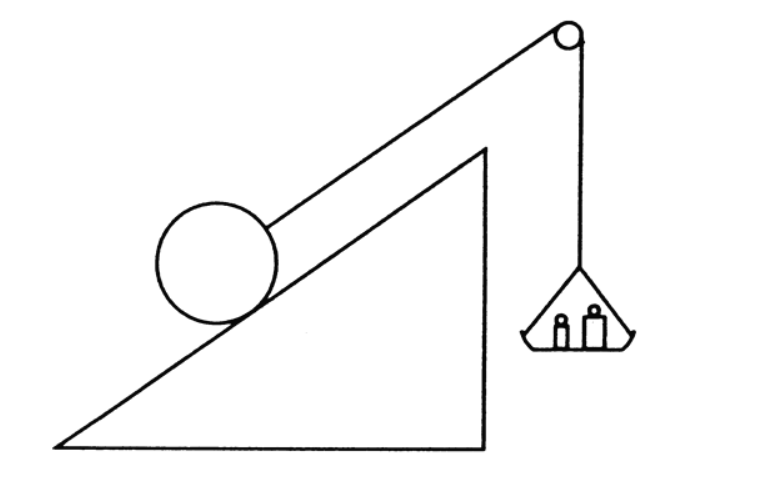
\includegraphics[scale=0.4]{Galileo1}

\subsection{Cronolog\'ia de la vida de Galileo}
\begin{description}
    \item 1564 - Nace en Pisa.
    \item 1581 - Comienza sus estudios de medicina en la Universidad de Pisa.
    \item 1585 - Se marcha de Pisa sin t\'itulo para vivir con su familia en Florencia.
    Empieza a dar clases.
    \item 1589  - Obtiene el puesto de profesor de matem\'aticas en la Universidad de Pisa.
    \item 1590  - Escribe De Motu.
    \item 1592 - Obtiene el prestigioso puesto de profesor de matemáticas en la Universidad de Padua.
    \item 1609 - El telescopio llega a Italia y es perfeccionado por Galileo.
    \item 1610 - Publica El nuncio sideral con gran éxito. Se traslada de Padua a Florencia bajo el mecenazgo del gran duque Cosme II.
    \item 1611 - Realiza una demostración de su nuevo telescopio en Roma.
    \item 1614 - Es atacado públicamente por la iglesia.
    \item 1616 - La iglesia le prohíbe «mantener o defender» el sistema copernicano.
    \item 1623 - Publica El ensayador. Maffeo Barberini se convierte en el papa Urbano VIII y permite a Galileo escribir un libro sobre las dos cosmologías rivales.
    \item 1632 - Tras ocho años de trabajo publica el Diálogo sobre los dos máximos sistemas del mundo. La iglesia le convoca a Roma.
    \item 1633 - El tribunal de la Inquisición le condena a cadena perpetua. Se retracta de su «ciencia herética».
    Vive bajo arresto domiciliario el resto de su vida.
    \item 1638 - El manuscrito de Discursos sobre dos nuevas ciencias es llevado clandestinamente a Holanda, donde se publica.
    \item 1639 - Se queda completamente ciego.
    \item 1642 - Muere a los 77 años.
\end{description}

\begin{thebibliography}{1}
\bibitem{[1]} Altshuler, J. (2002). \emph{A prop\'osito de Galileo.} M\'exico: Secretar\'́ia de Educaci\'on P\'ublica.
\bibitem{[2]} Strathern, P. (2017). \emph{Cienti\'ificos en 90 minutos.} Pack 1. Madrid: Siglo XXI de España Editores, S.A. 

\bibitem{a} \emph{Latex-Tutorial.} (2018). Consultado desde https://www.latex-tutorial.com
\bibitem{b} \emph{ShareLatex.} (2018). Consultado desde https://www.sharelatex.com/learn
\bibitem{c} \emph{Sascha-Frank.} (2018). Consultado desde http://www.sascha-frank.com
\bibitem{[7]} \emph{Alineación de párrafos.} (2018). Consultado desde https://latextips.wordpress.com/2009/01/27/alineacion-de-parrafos/

\end{thebibliography}
\end{document}






